\section{Pr�sentation de l'entreprise}

\begin{frame}{Pr�sentation de l'entreprise}
    \begin{block}{Activit�}
        \begin{itemize}
            \item Recherche \& D�veloppement
            \item Gestion de collections
            \item Fourniture de logiciels m�tiers
        \end{itemize}

    \end{block}
    
    \begin{block}{Cadre de travail}
        Collaboration avec l'�quipe de d�veloppement
    \end{block}

\end{frame}

%%

\section{Pr�sentation du sujet de stage}

\subsection{Le sujet}
\begin{frame}{Architecture actuelle}
	\centering
    \begin{textblock*}{2cm}(0.35cm,-2.65cm)
        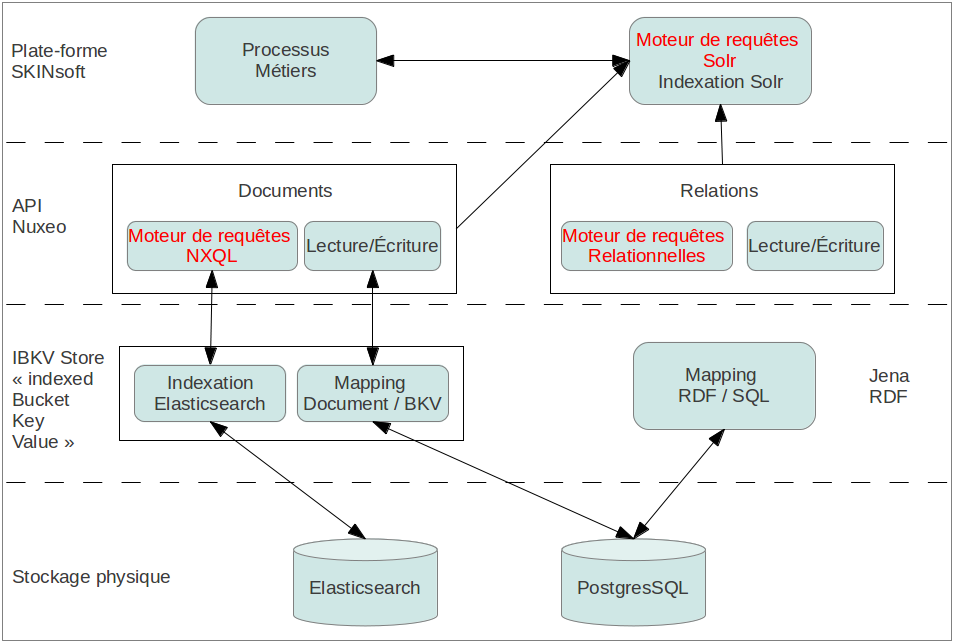
\includegraphics[scale=0.4]{./images/archi_evolution_skin}
    \end{textblock*}

\end{frame}

\begin{frame}{Architecture souhait�e}
	\centering
    \begin{textblock*}{2cm}(0.35cm,-2.65cm)
        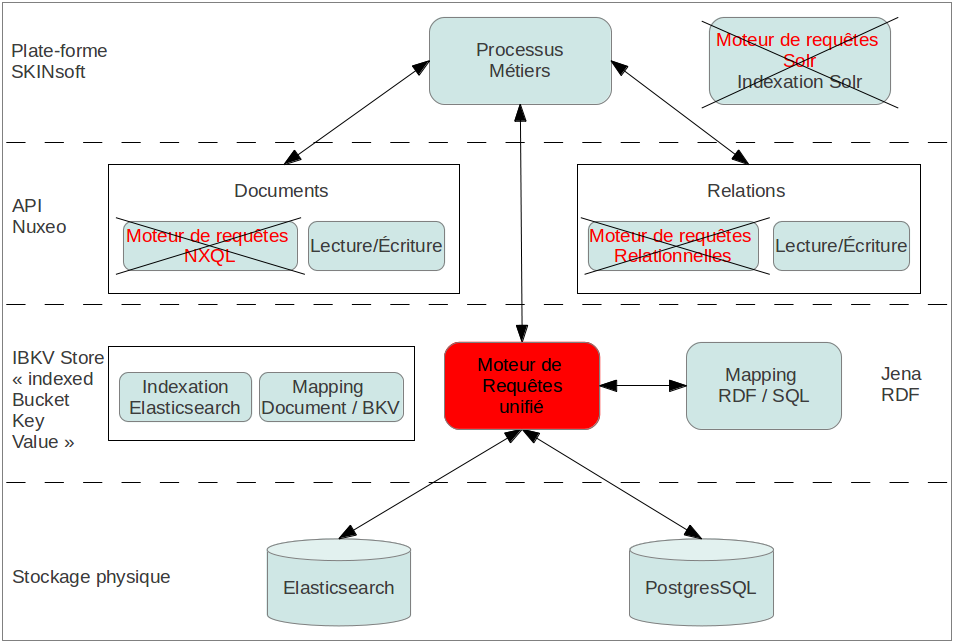
\includegraphics[scale=0.4]{./images/archi_unification_skin}
    \end{textblock*}

\end{frame}

%

\subsection{Probl�matique et d�marche}

\begin{frame}{Probl�matique}
    \begin{block}{{\'E}tat actuel}
        \begin{itemize}
        	\item Sources de donn�es h�t�rog�nes (documents, relations)
        	\item Langage NXQL existant non adapt�
        \end{itemize}

    \end{block}
    
    \begin{block}{Objectif}
        Ecriture d'un moteur de requ{\^e}tes unifi�
    \end{block}

\end{frame}

\begin{frame}{D�marche}
    \begin{block}{}
        \begin{enumerate}
        	\item {\'E}tude pr�liminaire de Elasticsearch
        	\item Impl�mentation du moteur de requ{\^e}tes
        	\begin{itemize}
        		\item Extension du langage de requ{\^e}tes existant
        		\item Mise en place de trois strat�gies diff�rentes
        	\end{itemize}
        \end{enumerate}
    \end{block}

\end{frame}



